\documentclass{article}

% packages
\usepackage[english]{babel}
\usepackage[utf8]{inputenc}
\usepackage{amsmath}
%\usepackage{amssymb}
%\usepackage{amsthm}
\usepackage{braket}
\usepackage{graphicx}
%\usepackage{bbm}
%\usepackage{multirow}
\usepackage{tikz}
\usetikzlibrary{positioning}
\usetikzlibrary{shapes.arrows}
\usepackage{color}
%\usepackage[colorinlistoftodos]{todonotes}
%\usepackage[absolute,overlay]{textpos}
%\usepackage{hyperref} % Should be last package imported
\usepackage{fullpage}

%%%%%%%%%%%%%%%%%%%%%%%%%%%%%%%%%%%%%%%%%%%%%%%%%
%%% SHORTCUTS %%%

%\newcommand{\pagehline}{\\\specialrule{.01pt}{0pt}{5pt}}
\newcommand{\pagehline}{\noindent\rule{\textwidth}{0.2pt}}

\newcommand{\paren}[1]{\left( #1 \right)}
\newcommand{\expectation}[1]{\left< #1 \right>}
\newcommand{\brac}[1]{\left[ #1 \right]}
\newcommand{\zerodel}{.\kern-\nulldelimiterspace}
\newcommand{\abs}[1]{\left\vert #1 \right\vert}
\newcommand{\wt}[1]{\widetilde{#1}}

\newcommand{\vecE}{\mathbf{E}}
\newcommand{\vecB}{\mathbf{B}}
\newcommand{\kvec}{\mathbf{k}}
\newcommand{\xvec}{\mathbf{x}}
\newcommand{\rvec}{\mathbf{r}}
\newcommand{\bvec}{\mathbf{b}}
\newcommand{\Rvec}{\mathbf{R}}
\newcommand{\zbar}{\overline{z}}
\newcommand{\curl}{\nabla\times}
\renewcommand{\div}{\nabla\cdot}

\DeclareMathOperator{\Lagr}{\mathcal{L}}
\DeclareMathOperator{\Ham}{\mathcal{H}}
\DeclareMathOperator{\tr}{tr}

\newcommand{\lucas}[1]{\textcolor{blue}{\bf [LKW #1]}} % Lucas comment


\begin{document}

\begin{center}
{\Large Fitting a band structure model for silicon}
\end{center}

\section{Mean field calculation}

A conventional silicon cell was used (diamond structure) with 8 Si atoms (16 up electrons, 16 down).
Kohn-Sham orbitals were computed at the gamma point using DFT.
DFT was run in PySCF using the PBE xc-functional and BFD pseudopotentials.
(Exponents less than $0.1$ were removed.)
There are 16 occupied orbitals in the lowest energy mean-field wave function.


\section {Low energy states}

To describe the low energy degrees of freedom, we choose determinants corresponding to low energy mean-field excitations.
The DFT orbital energies are shown in Fig \ref{fig:dft_energies}.

\begin{figure}[h]
\begin{center}
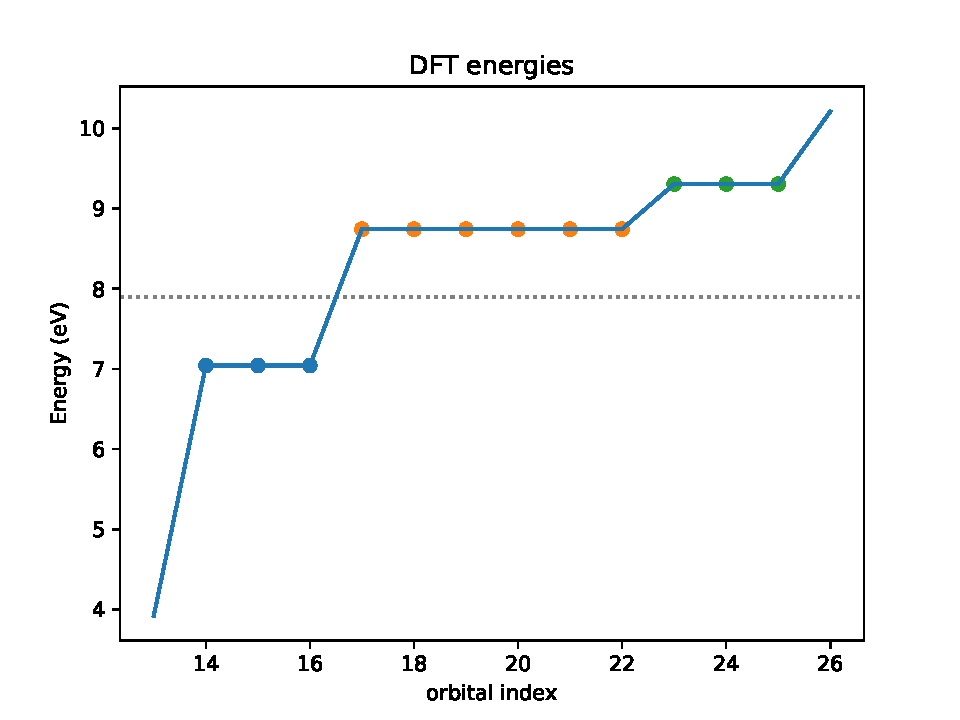
\includegraphics[width=0.5\textwidth]{images/dft_energies_k888.pdf}
\label{fig:dft_energies}
\caption{DFT orbital (single particle) energies. 
Dots are the orbitals used to generate excitations. 
Dotted gray line is the Fermi energy.}
\end{center}
\end{figure}

The states sampled for the model are combinations of Slater determinants multiplied by a Jastrow factor.
The Slater determinant part is defined as

\begin{equation}
\Psi^S = \sum_i c_i D_i,
\end{equation}

where each Slater determinant $D_i$ is chosen by promoting electron(s) from an occupied orbital to an empty orbital.
The weights $c_i$ are normalized, so the number of tunable parameters is one less than the number of determinants.

The final wave function has the form

\begin{equation}
\Psi = \Psi^S \Psi^J,
\end{equation}

where the Jastrow factor $\Psi^J$ is optimized to minimize the energy given the nodal structure of $\Psi^S$.
This is done to project out the components of the wave function not in the desired low-energy subspace.

\subsection{Choosing excitations}

\begin{figure}[h!]
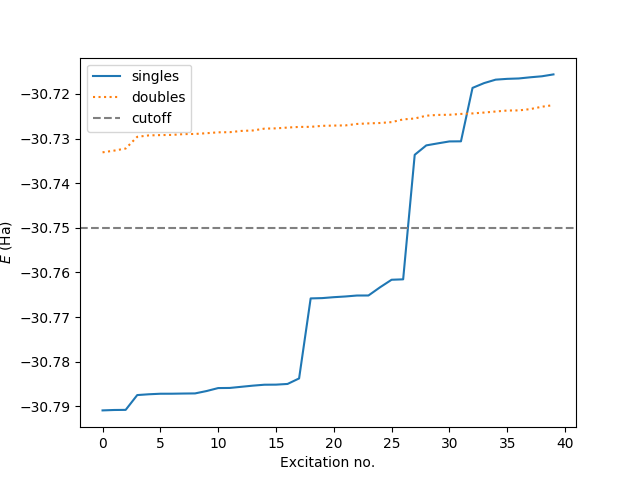
\includegraphics[width=0.5\textwidth]{images/determinant_mf_energies.png}
\label{fig:energy_cutoff}
%TODO update old data!
\caption{\textcolor{red}{\bf !!OLD DATA!!} Mean-field DFT total energies for singles and doubles excitations.
The dashed line shows the cutoff chosen for the samples used in this calculation.}
\end{figure}

To fit a ``low energy'' model, it is ideal to choose states below an energy gap so that the states are well described by the low energy subspace of the Hilbert space.
(If there is no gap, the states may have components not included in the low energy space, introducing energy variance that is not relevant to the model.)
We choose an energy cutoff in the gap shown in Fig \ref{fig:energy_cutoff}, which only includes singles excitations.

\subsection{Wave function samples}

The model we consider here assigns energies to the molecular orbitals,

\begin{equation}
E = \epsilon_0 + \sum_i \epsilon_i n_i,
\end{equation}

where $i$ indexes a set of molecular orbitals, and the orbital energies $\epsilon_i$ are model paramaters that are fit to the QMC data.
In this set of samples, a total of 12 orbitals have varying occupation (three valence, nine conduction, Fig \ref{fig:descriptors}).
Since the total number of electrons is constant, there are only 11 degrees of freedom in the orbital occupations.

\begin{figure}[h!]
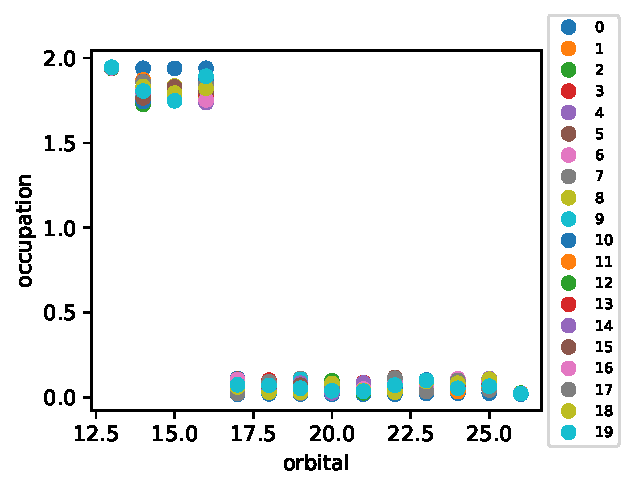
\includegraphics[width=0.5\textwidth]{images/dmc_lowen_descriptors.pdf}
\label{fig:descriptors}
\caption{Occupation of orbitals for different samples. Each color is a sample, orbital index varies along the x-axis.}
\end{figure}

The correlation matrix of the descriptors shows how the energy is correlated with the orbital occupations (Fig \ref{fig:descriptors_corrmat}).
The correlation samples include both the values and derivatives of the energies and occupations.
Since there is a constant term in the model, the mean of the energies was subtracted off (but not of the derivatives).
As we should expect, the energy is negatively correlated with the valence occupations, and positively correlated with the conduction occupations.

\begin{figure}[h!]
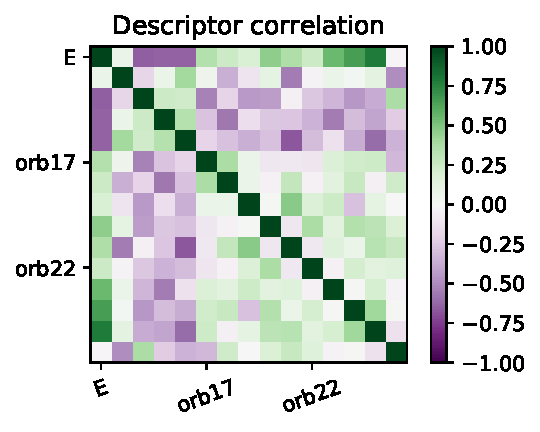
\includegraphics[width=0.5\textwidth]{images/dmc_lowen_corrmat.pdf}
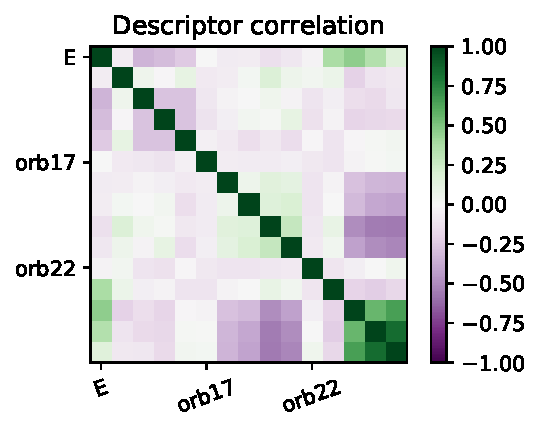
\includegraphics[width=0.5\textwidth]{images/dmc_allderivs_lowen_corrmat.pdf}
\label{fig:descriptors_corrmat}
\caption{
Left: The correlation matrix (DMC) of the energies and orbital occupations (not including derivatives). 
Right: The correlation matrix (DMC) of the energies and orbital occupations, including derivatives.}
\end{figure}

\subsection{Fitting a model}

The model is fit by linear regression.

\begin{figure}[h!]
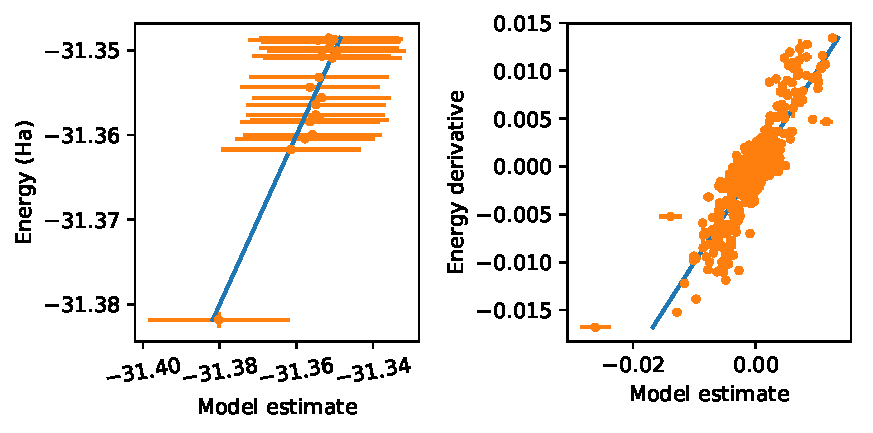
\includegraphics[width=0.5\textwidth]{images/dmc_allderivs_lowen_model.pdf}
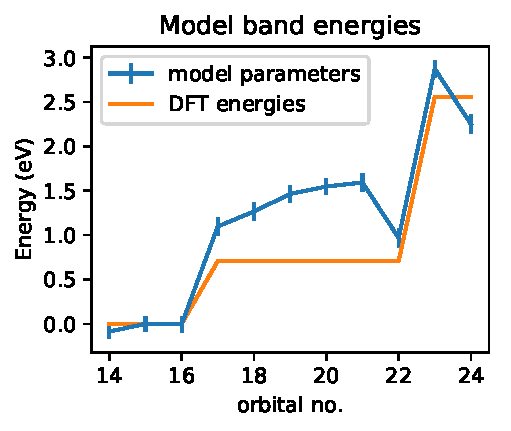
\includegraphics[width=0.5\textwidth]{images/dmc_allderivs_lowen_model_bands.pdf}
\label{fig:model_fit}
\caption{Model fit with derivatives. 
Left: Plot of data vs model prediction. 
Right: The orbital energies of the model, corresponding to shifted DFT energies.}
\end{figure}

  
  




\end{document}
